% !TeX spellcheck = en_GB
% !TeX root = Report.tex
\phantomsection
\addcontentsline{toc}{section}{Conclusions}
\sect{Conclusions}

A number of companies with varying patent strategies have been considered.
They are categorised in the Patent-Success Synergy Matrix in figure~\ref{fig:pssm:companies}.
Here, the categories are not boolean - but on a scale. 
The $x$ axis represents the patenting strategy from few to many.
The $y$ axis is proportionate to the success. 
The more successful the compnay is, the further up the company is represented on the matrix.
%\todo[inline]{Explain the matrix with scale - when it's made!}
\begin{figure}[!h]
\centering
%\missingfigure{Use figure \ref{fig:synergymatrix} with companies added}
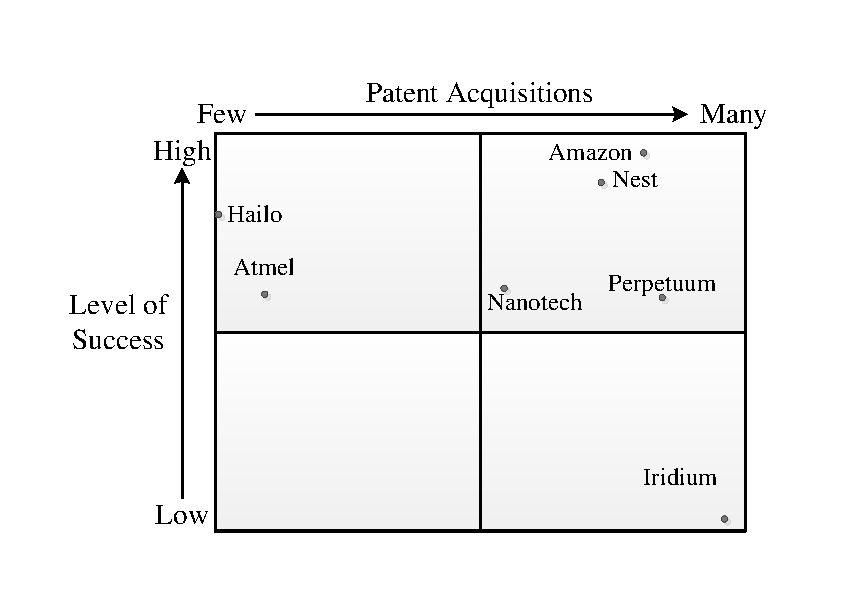
\includegraphics{Figures/SuccessMatrixScale.pdf}
\caption{Patent-Success Synergy Matrix with companies}%\todo[inline]{Nanotech to be moved to less patents. Whole figure to be flipped so many patents is on right.}}
\label{fig:pssm:companies}
\end{figure}

In this situation, it is difficult to compare HAILO to the other companies. 
This is due to them both being software orientated. 
As discussed in the introduction, software is difficult to patent, and so does not provide a good comparison to the other, hardware orientated companies.

Atmel were verging on the line of failure/success in their early days. 
They managed to recover their business after accusations from Intel to form a very good company, with patents in place to protect them.


Iridium, Nest, Perpertuum and Amazon all show a similar strategy - they were all first to market with their inventive idea.
The acquisition of patents for these companies was key as it allowed them to gain a monopoly over their market. 
All three companies had good, inventive technology.
Nest and Perpetuum became successes with the future looking bright for the younger Perpetuum. 
They both hold good standings in their markets with the needed legal defence to help them.
Iridium, however, had a good idea, and the patents to back their venture. 
But due to a large amount of new technology to realise their goal, and unreliable hardware meant customers were put off.
The company put a large amount of effort into their product without the certainty of customers or success. 
If the company was successful, the patents would have been a great aid to give them exclusivity to their market.

Nanotech are an exception, to some extent.
They hold very few patents \cite{nanotechpatent} but still remained successful as they were bought out by Gennum Corporation. 
This could be due to the fact they were not the first to the market, or that they managed to develop a product that was the best available. 
By filing for a patent, they would have to disclose the workings of their device, whereas the company may have wished to keep it a trade secret.

It is clear that if you are first to market, patents are extremely valuable as they give you a monopoly over the market. 
This removes a large amount of the competition until a company develops a similar technology which does not violate patents, and out performs the existing product. 
However, this is difficult to do as by the time such a product is made, the market holder would be well established with good customer relations.

Patents are not the golden key to success. 
Holding good patents is not an excuse to neglect basic entrepreneurialism and business strategy. 
There is a large lesson to be learnt from Iridium's failure for all emerging companies.
It is also not necessary to hold many patents to be successful either.
Atmel managed their early life without patents, and therefore were flexible in their R\&D to develop a product. 
Their memory won the market not out of exclusivity, but from good performance and business strategy.

In conclusion, the acquisition of patents is a tricky, but important decision to make.
Patents should be acquired where needed to give exclusivity.
They add value to a company, as well as defence against other companies copying a product.
However, patents are not an alternative to the basic business strategy and skills needed to be successful.



